\section{LOGICAL MODEL STRUCTURE}\label{sec:dataware}

The logical model of the data warehouse is a snowflake schema as shown in Figure \ref{fig:datawarehouse}. It consists of 8 tables, 3 of those being fact tables. Additional information tables are called support tables in the system. These describe surrounding information necessary to build the fact tables. Trivial dimensions like Date and Time will not be described in depth. The color encoding is as following; Purple entities reside solely with the customer, while both customer and insurance company have access to the red entities. The green entity is only used situationally, but available to both parties when agreed upon. The reasoning behind this will be described in depth in the next paragraph.

\begin{figure*}[tb]
\centering
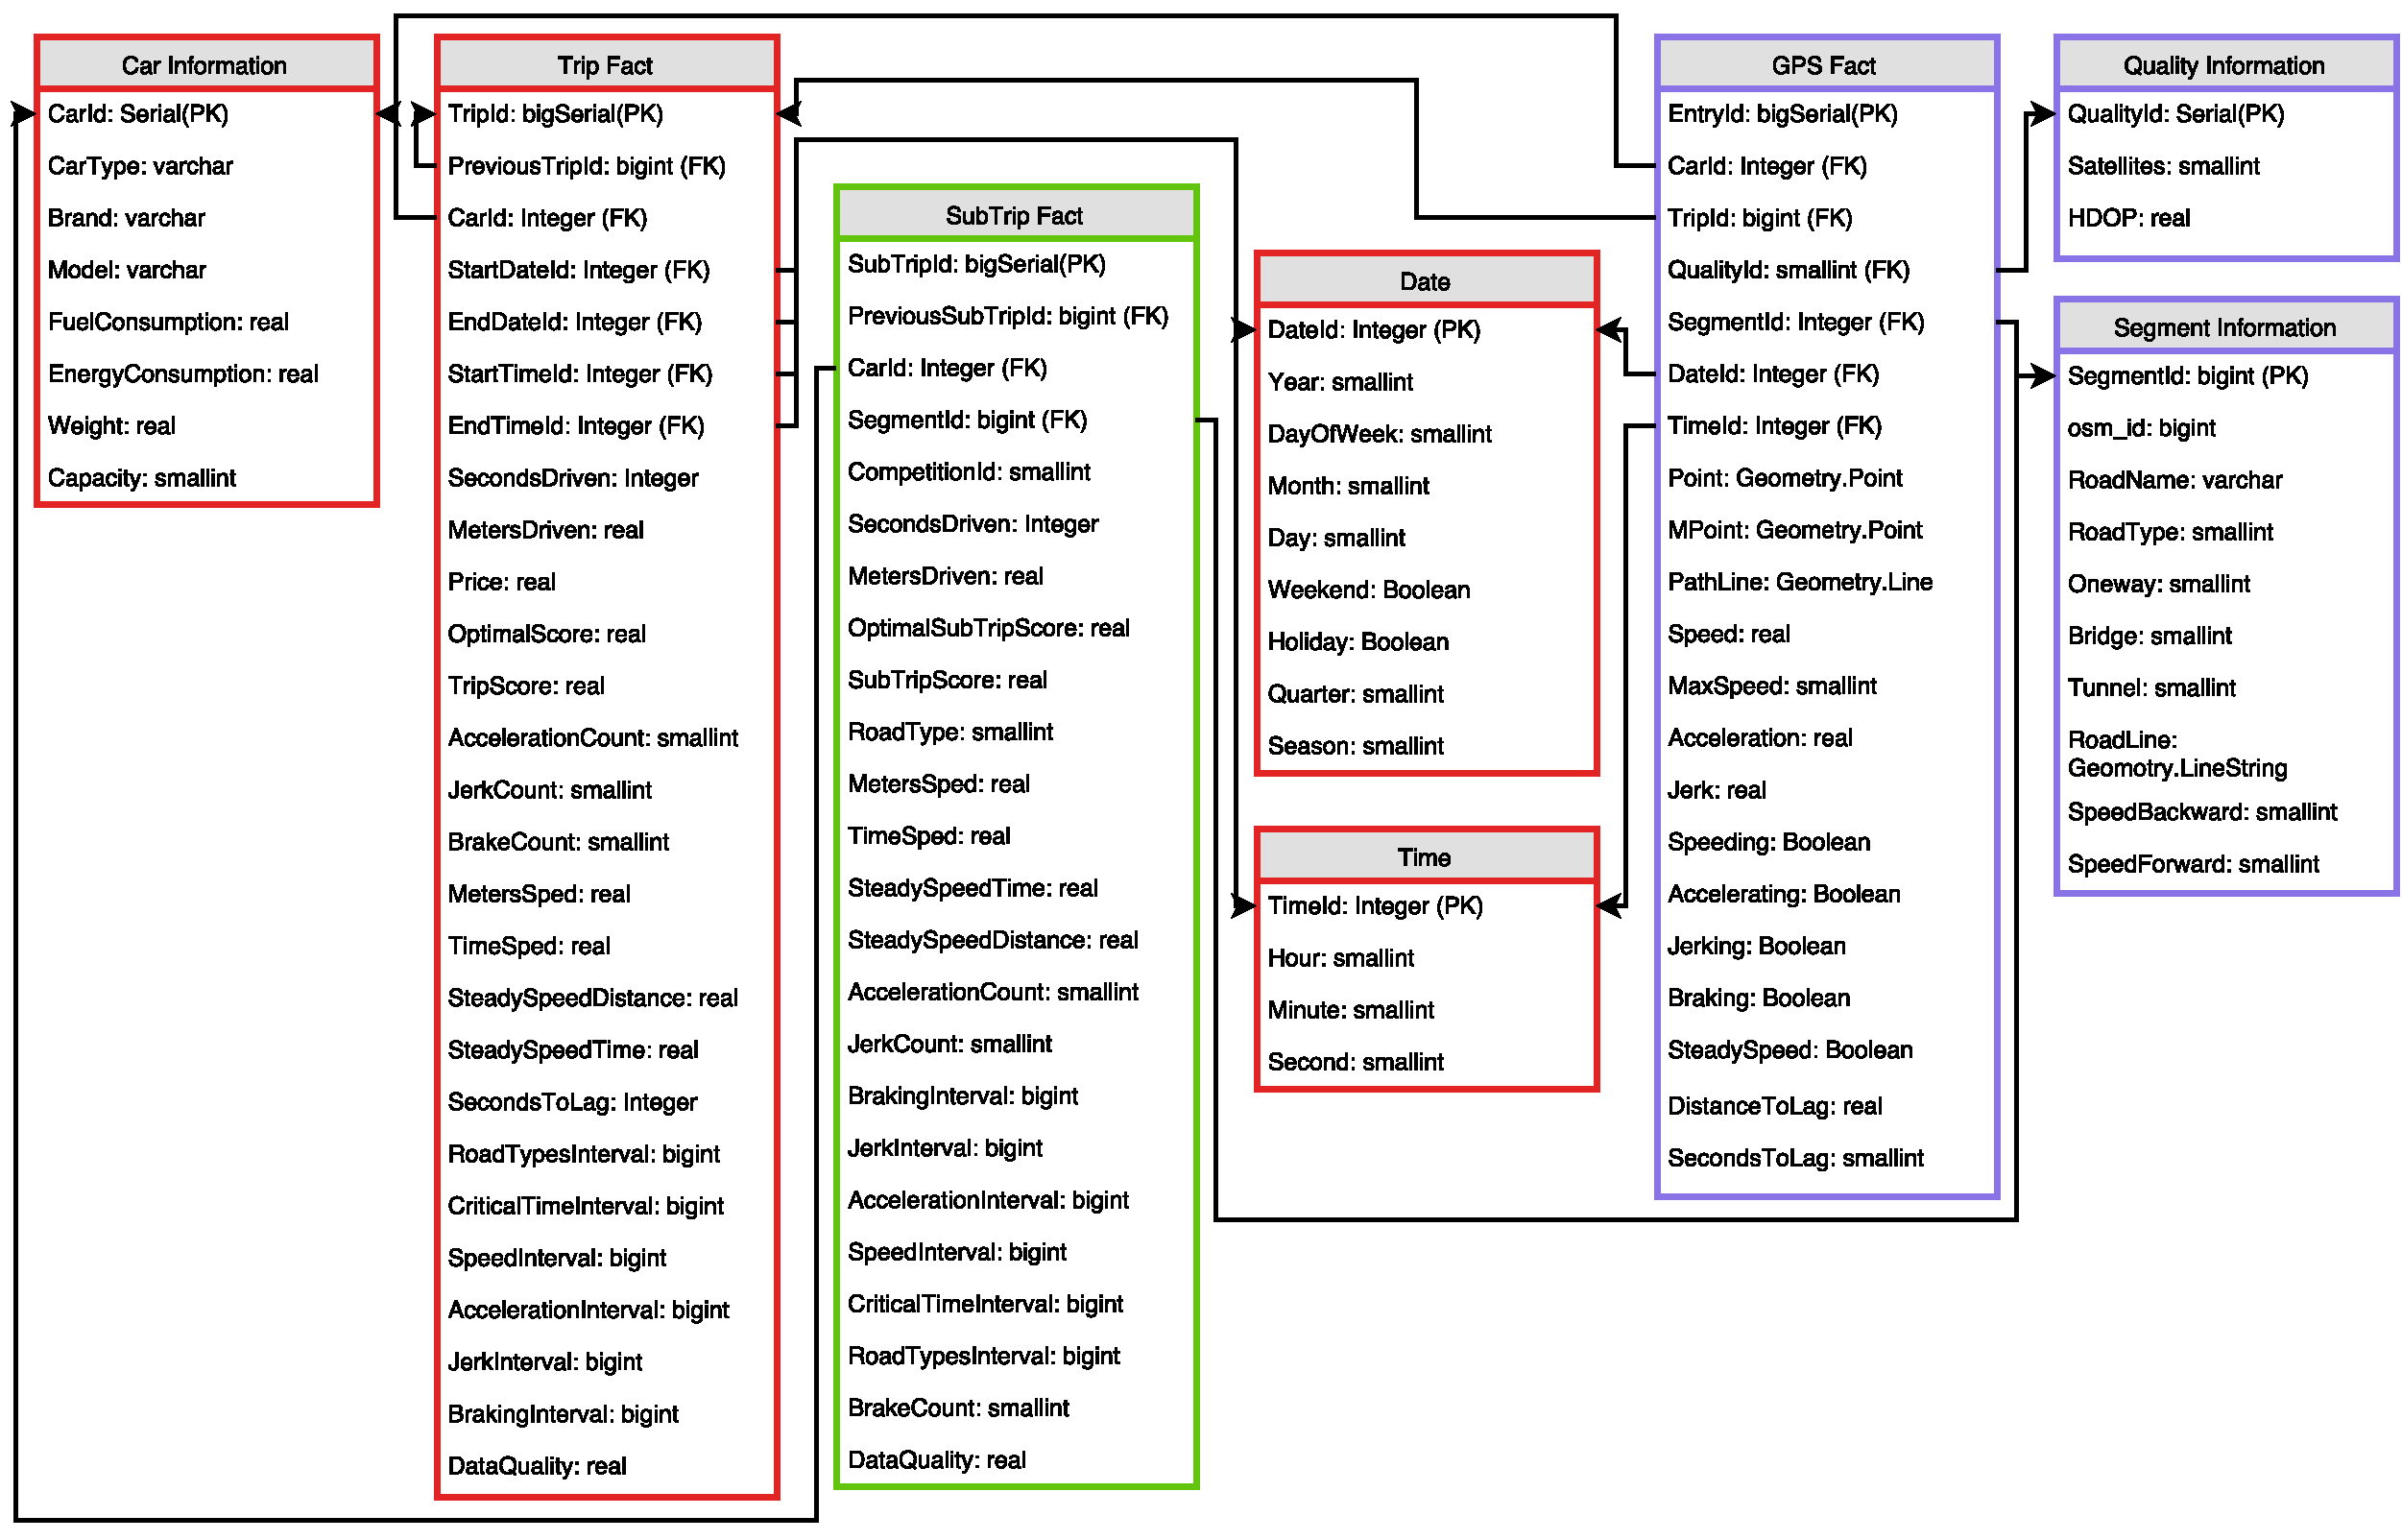
\includegraphics[width=0.9\textwidth]{Pictures/ERDiagram}
\caption{Logical Model of the Data Warehouse}
\label{fig:datawarehouse}
\end{figure*}

\subsection{Fact Tables}
Amongst the fact tables an implicit hierarchy is present. The gpsfact table is the main fact table where raw data is stored through the logging device. Certain measures are calculated on the logged entry, and added to the database. After trips are ended, a tripfact is created using data from the gpsfacts. tripfacts store general information about the trip and is as such on the highest level of the hierachy. Similar to tripfacts, Subtripfacts are calculated from collections of gpsfacts, but at a finer granularity. A single subtripfact is associated with a single segment that a car has driven on. Representing an entire trip with subtripfacts will as such require one row per segment. The interaction between tables and process of storing GPS data will be further described in \nameref{sec:ETL}. 

\textbf{GPS Fact} is the center of the entire data warehouse. Each entry represents a singular GPS point of a car, with a reference to the date and time for which it was recorded. The table references all of the support tables, as well as a reference to a single tripfact. A gpsfact contains the spatial attributes \textit{Point}, \textit{MPoint} and \textit{PathLine}, which respectively are raw GPS coordinates, map-matched GPS coordinates and a line to the previous GPS coordinate. A gpsfact contains several boolean values, namely \textit{Speeding}, \textit{Accelerating}, \textit{Jerking}, \textit{Braking} and \textit{SteadySpeed}. These act as an indicator for an ongoing event, identified from the name. They are purely used for convenience in querying, as the actual value can be extracted from the measures themselves. The actual values of the attributes are all calculated in relation to the previous points, e.g. acceleration is the change in speed between the current and previous gpsfact, divided with the distance between them.

\textbf{Trip Fact} entries represents a logical car trip through a collection of GPS coordinates. They contain a start-time and an end-time represented by 4 foreign keys to the Date and Time dimensions. A tripfact has many attributes which summarizes data collected through the gpsfacts. These are \textit{MetersDriven}, \textit{SecondsDriven} and all of the count attributes. Each trip fact has a \textit{TripScore} and \textit{OptimalScore} which are calculated scores, given an active insurance policy. Scores and associated calculations are described later in \ref{sec:trip}. A contribution of this paper is the decision create intervals in the form of a bigInt, to represent to the degree of delinquencies. To explain this further, consider the example in Table \ref{tab:intervalexample} with accelerations logged during a trip; 

\begin{table}[h]
\centering
\begin{tabular}{cc | cc}
\multicolumn{2}{c}{\textbf{Policies}} & \multicolumn{2}{c}{\textbf{Logged Info}} \\\hline
\textbf{Intervals ($m/s^{2}$)}     & \textbf{Weights}     & \textbf{Amount}     & \textbf{Percentage}     \\\hline
{[}3, 4 {[}              & 1.05              &   32            & 40              \\
{[}4, 4.5 {[}            & 1.10              &   16            & 20              \\
{[}4.5, 5 {[}            & 1.15              &   8             & 10              \\
{[}5, 5.5 {[}            & 1.25              &   4             & 5              \\
{[}5.5, 6 {[}            & 1.35              &   8             & 10              \\
{[}6, 6.5 {[}            & 1.45              &   4             & 5              \\
{[}6.5, 7 {[}            & 1.55              &   8             & 10              \\
{[}7, $\infty$ {]}       & 1.80              &   0             & 0              \\\hline
\end{tabular}
\caption{An example of accelerations and intervals}
\label{tab:intervalexample}
\end{table}

All of the accelerations for this trip are divided into different intervals depending on their severity. Both the intervals and their associated weight are determined by some policy created by the insurance company. In effect, the insurance company can decide exactly when a metric is important. By example, table \ref{tab:intervalexample} excludes everything from 0m/s to 3m/s, and considers everything above 7m/s as bad as it gets. Intervals between these values are chosen to have a finer granularity.

It is possible to have different policies throughout the system, as the policy in question is represented by the 2nd and 3rd digit in the bigInt. This provides a maximum of 100 unique policies. The intervals representing delinquencies also have two digits for representation. Raw counts can however easily extend past 100. To remedy this we save the percentage of total delinquencies instead, and save the total count separately. This however creates an edge case of single interval containing 100\% of the registered delinquencies, thus requiring 3 digits. This is remedied by setting the 1st digit of the bigInt to 1. When a 1 is read on the first position it is then understood that the first non-zero interval is 100\%. Parsing the data in table \ref{tab:intervalexample} would result in the following bigInt given a policy ID of 01

$$
0\ 01\ 32\ 16\ 08\ 04\ 08\ 04\ 08\ 00 \eqno{(1)}
$$

\textbf{SubTrip Fact} is a special fact table in the sense that it does not have any direct impact on the billing scheme. It is created with gamification in mind, allowing customers to part with some of their private data. This can allow direct comparison to other drivers, making it possible for the insurance company and possibly others to make competitions and games based on the data of customers.
A subtripfact is created for every segment on a trip, making it possible to directly compare, not only for entire trips, but also for specific sequences of segments. Aside from only covering a certain segment, the subtripfact table is very similar to the Trip Fact. Direct comparison between full tripfacts are hard though because longer routes are usually quite unique. 

The subtripfact table is empty by default, and only used when customers engage in some element of gamification. As such the customer will never give away privacy-intruding data without knowledge. This has to be emphasized because subtripfacts are sketchy in terms of customer privacy.

A noticable difference between tripfacts and subtripfacts is the \textit{competitionId}. This ID is what makes it possible for the insurance company to associate competitions and games with certain segments. An example of a competition could be as follows:
The customer with the best record on the street Vesterbro, between January 1st and February 1st, gets 5\% off on their insurance costs. When the insurance company has issued the competition, the customer can sign up. The system calculates a subtrip for every time the customer has traversed the given segment(s). Given the privacy-sensitive data involved, the sign up would have to include the customer to sign a Terms-Of-Service, agreeing to handing over data that might be privacy intrusive. 

\subsection{Support Tables}
\textbf{Car Information} is a support table holding information about the insured car. The data is valuable to the insurance company, if not for actual insurance calculations, then for statistical use. The data has a relation 1 to many tripfacts, subtripfacts and gpsfacts, meaning each of these must have be linked to an actual car. This is important since the insurance policy is per car, rather than per person.

\textbf{Quality Information} is a support table which determines the quality of associated gpsfacts. The table contains information on the Horizontal-Dilution-of-Position (HDOP) and the amount of satellite used to measure the position of the car. Whenever a new combination of HDOP and satellite count is seen, a new entry is created in the database. Entries are mapped as 1 to many gpsfacts, reducing the amount of duplicated information in the database.

\textbf{Segment Information} contains the entire road network of Denmark, originating from OpenStreetMap. The osm\_id  attribute is the global ID OpenStreetMap uses to identify a specific segment. It is kept to make it possible for cooperation and better integration in the future. Segment Information has a 1 to many relationship with both subtripfacts and gpsfacts.